\documentclass[10pt,a4paper]{article}

\usepackage{fullpage}
\usepackage{setspace}
\usepackage{parskip}
\usepackage{titlesec}
\usepackage[section]{placeins}
\usepackage{xcolor}
\usepackage{breakcites}
\usepackage{lineno}
\usepackage{hyphenat}

\setlength\columnsep{25pt}





\PassOptionsToPackage{hyphens}{url}
\usepackage[colorlinks = true,
            linkcolor = blue,
            urlcolor  = blue,
            citecolor = blue,
            anchorcolor = blue]{hyperref}
\usepackage{etoolbox}
\makeatletter
\patchcmd\@combinedblfloats{\box\@outputbox}{\unvbox\@outputbox}{}{%
  \errmessage{\noexpand\@combinedblfloats could not be patched}%
}%
\makeatother


\usepackage{natbib}




\renewenvironment{abstract}
  {{\bfseries\noindent{\abstractname}\par\nobreak}\footnotesize}
  {\bigskip}

\titlespacing{\section}{0pt}{*3}{*1}
\titlespacing{\subsection}{0pt}{*2}{*0.5}
\titlespacing{\subsubsection}{0pt}{*1.5}{0pt}


\usepackage{authblk}


\usepackage{graphicx}
\usepackage[space]{grffile}
\usepackage{latexsym}
\usepackage{textcomp}
\usepackage{longtable}
\usepackage{tabulary}
\usepackage{booktabs,array,multirow}
\usepackage{amsfonts,amsmath,amssymb}
\providecommand\citet{\cite}
\providecommand\citep{\cite}
\providecommand\citealt{\cite}
% You can conditionalize code for latexml or normal latex using this.
\newif\iflatexml\latexmlfalse
\providecommand{\tightlist}{\setlength{\itemsep}{0pt}\setlength{\parskip}{0pt}}%

\AtBeginDocument{\DeclareGraphicsExtensions{.pdf,.PDF,.eps,.EPS,.png,.PNG,.tif,.TIF,.jpg,.JPG,.jpeg,.JPEG}}

\usepackage[utf8]{inputenc}
\usepackage[ngerman,english]{babel}



\usepackage{float}



\usepackage[margin=1.5in]{geometry}




% Edit this header.tex file to include frontmatter definitions and global macros

% Add here any LaTeX packages you would like to load in all document blocks
% \usepackage{xspace}
\usepackage{dcolumn}

% Add here any LaTeX macros you would like to load in all document blocks
% \def\example{This is an example macro.}

\newcommand{\beginsupplement}{%
        \setcounter{table}{0}
        \renewcommand{\thetable}{A\arabic{table}}%
        \setcounter{figure}{0}
        \renewcommand{\thefigure}{A\arabic{figure}}%
     }

% -----

\iflatexml
% Add here any LaTeXML-specific commands

% -----

\else
% Add here any export style-specific LaTeX commands. These will only be loaded upon document export.
% \paperfield{Subject domain of my document}
% \keywords{keyword1, keyword2}
% \corraddress{Author One PhD, Department, Institution, City, State or Province, Postal Code, Country}
% \fundinginfo{Funder One, Funder One Department, Grant/Award Number: 123456.}
\fi


\begin{document}

\title{Does the Belt and Road Initiative Promote the Economic Growth of
Developing Countries?}



\vspace{-1em}



  \date{\today}


\begingroup
\let\center\flushleft
\let\endcenter\endflushleft
\maketitle
\endgroup


\linenumbers



\onehalfspacing


\selectlanguage{english}
\begin{abstract}
The Belt and Road Initiative (BRI) is an infrastructure-led global
development program proposed by China in 2013. This paper exploits the
impact of the BRI on the economic growth of its member countries in the
developing world. A difference-in-difference approach shows that the
BRI-induced investment on average increased the recipient countries'
real GDP by 5\% compared to their counterparts at similar levels of
development. The study also suggests that the BRI investment helps these
countries to industrilize by increasing their industrial value-added by
almost 13\%.~%
\end{abstract}%




\section{Introduction}

{\label{921879}}

The Belt and Road Initiative (BRI) is China's ambitious global
development program that was initially proposed by President Xi Jinping
in 2013. The program involves a vast number of countries across Asia,
Europe, and Africa, which covers 65\% of the world population, and 40\%
of the world's GDP as of 2017~\hyperref[csl:1]{(Campbell 2017)}. The BRI is featured by
massive infrastructure investment along the ``belt'' and the ``road'' to
improve the cross-border connectivity and promote trade and economic
prosperity (Figure~{\ref{885875}}).~

\par\null\selectlanguage{english}
\begin{figure}[H]
\begin{center}
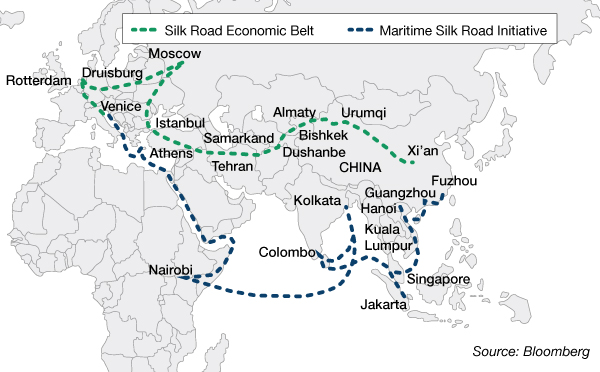
\includegraphics[width=0.70\columnwidth]{figures/map3/map3}
\caption{{The ``Belt'' and the ``Road''
{\label{885875}}%
}}
\end{center}
\end{figure}

This paper seeks to answer the question: do the countries joining the
BRI actually benefit from this program and by how much? To answer this
question, I evaluate the impact of the BRI investment on its recipient
countries' economic performance by using a staggered
difference-in-difference approach on a matched sample. The main finding
is that the investment induced by the BRI increased the real GDP of the
member countries by 5\% on average compared to their counterparts at
similar levels of development. The increased output was driven by a 5\%
increase in agricultural value-added and a nearly 13\% increase in
industrial value-added.~

There are two main challenges to obtain a causal interpretation when
studying the effect of infrastructure investment and economic growth.
The first is the huge heterogeneity between countries and the complex
nature of economic growth. It is hardly persuasive to conclude anything
by simply comparing countries that are vastly different in culture,
demography, institutions, and levels of development. The second
challenge is that infrastructure is often considered endogenous to the
process of economic growth. A natural concern is that the investment is
subject to selection -- China may select to invest in those countries
with growth potential.~

To address the first concern, I conduct a propensity score matching
before any further exploration. I construct a control group that is
similar to the treatment group in average GDP per capita, GDP growth
rate, and levels of industrialization before the BRI. Then a standard
staggered difference-in-difference analysis is conducted on the matched
sample. A set of fixed effects is controlled throughout the study to
filter out any time-invariant confoundings that could influence economic
growth such as language, culture, geographic location, resource
endowments, and so on. A set of time-varying covariates is also
controlled for robustness.~

To address the second concern, it would be ideal if an experiment could
be conducted in which the destination and timing of the infrastructure
investment are randomly assigned, though this is not feasible in
reality. However, the announcement of the BRI did induce investment
shocks to some of its member countries, in which the amount of
investment from China doubled or tripled after the BRI announcement in
2013. The policy-induced investment shocks can be regarded as
quasi-random in timing for the recipient countries in the sense that it
drastically increased the amount of foreign direct investment (FDI) to a
level that would not be expected in natural courses of events, and such
investments would not happen had a less ambitious leader taken power in
China. I make use of this quasi-randomness and define a country as being
treated if it received significantly more FDI from China after joining
the BRI.~

The key identifying assumption is that, in the absence of BRI
investment, the average rate of GDP growth would have been the same for
both treated and untreated countries. By working on a matched sample,
there are no longer differences between the treated and untreated
countries on average before the treatment. And controlling both country
and year fixed effects~eliminate any time-invariant confounding factors
as well as common time trend caused by global economic~vicissitudes.
Additional robustness checks are also conducted to make sure the
parallel assumption holds and the result is not driven by omitted
variable bias, selection issues, or any other biases.

The rest of the paper is organized as follows.
Section~{\ref{494291}} briefly introduces the
background of the BRI and reviews the related literature.
Section~{\ref{436643}} describes the data sources and
the empirical strategy. Section {\ref{411455}}~presents
the main regression results of the difference-in-difference analysis.
Section~{\ref{351972}}~provides further robustness
checks. Section~{\ref{322007}} concludes.~

\par\null

\section{Background and Literature
Review}

{\label{494291}}

The Belt and Road Initiative was initially proposed by China's President
Xi Jinping during his visits to Kazakhstan and Indonesia in late 2013.
President Xi called for new models for regional cooperation and
development, by collaboratively building the so-called ``Silk Road
Economic Belt'' and the ``21st Century Maritime Silk Road''.~ The
initiative was therefore officially termed as the ``Belt and Road'' or
``One Belt One Road'' \hyperref[csl:2]{(Xinhua 2015)}.~

The ``Belt'' refers to an overland route analogous to the ancient Silk
Road that connects West China, Central Asia, West Asia, and Europe. The
``Road'' is a maritime route that goes through the South China Sea,
South Pacific Ocean, Indian Ocean, and onward to Africa and Europe
(Figure {\ref{885875}}).

The salient feature of the Belt and Road Initiative which distinguishes
it from other global cooperative programs is its emphasis on
infrastructure. The initiative plans to build a vast web of
infrastructure including cross-broader roads and railroads, oil and gas
pipelines, telecom and electricity links, seaports, and more. By heavily
investing in infrastructure, China seeks to ``enhance regional
connectivity and embrace a brighter future''\hyperref[csl:3]{(Xinhua 2015)}. From
2013 to 2018, China has invested more than 90 billion dollars in the BRI
countries, growing at a rate of 11.9\% annually~\hyperref[csl:4]{(Xinhua 2019)}. The
amount of investment would, as China says, total up to 4 trillion
dollars in the future.

The motivation behind this ambitious initiative has been the center of
the debate in the literature. Many strategists believe that it is
China's geostrategic move to increase its global influence and ``enhance
international political legitimacy as a global power and leader of the
Developing World''~\hyperref[csl:5]{(Scobell et al. 2018)}.~ It is also believed that there
are national security concerns that China seeks to secure its resource
and energy supply from Central Asia and the Middle East by enhancing
relations with the countries to its west and plan ahead for the risk of
strategic encirclement from the Pacific Ocean.~

Economic concerns are also the main driving forces behind the proposal.
While China's economic growth has been slowing down in recent years, the
BRI is considered one of the Chinese government's efforts to sustain its
economic growth~\hyperref[csl:6]{(Huang 2016)}. By helping BRI countries building
their infrastructure, China is exporting its excess capacity of steel,
coal, construction, and building materials. This helps China to sustain
its old industries while transitioning to innovation-led new industries
takes decades to come.

The BRI also serves as a development strategy for China's vast western
inland~\hyperref[csl:7]{(Yu 2016)}. China's vast western inland, which occupies
almost two-thirds of the national land, has long been suffering from
economic backwardness due to its landlocked disadvantage. Revitalize the
ancient Silk Road enables West China to participate directly in global
trade, and possibly turns it into a trade hub between China and other
Euroasia countries.

China has been one of the favorable destinations for global labor
outsourcing for decades. However, as its domestic labor cost being
steadily rising, China seeks to outsource some of its industries to
countries with even cheaper labor. This motivates China's state-owned
enterprises (SOEs) to help some countries improving their infrastructure
to pave the way for such industrial relocation. The political dialogue
along with the economic efforts also helps to reduce the policy risk and
uncertainty for Chinese firms to invest in these BRI
countries~\hyperref[csl:8]{(Du and Zhang 2018)}.~~

China also believes by helping other developing countries improving
their economic capability, it opens new markets for China's export
goods, which helps to sustain China's export-oriented manufacturing
industries. Since the launching of the initiative, China's trade volume
with the BRI countries reached 1.3 trillion dollars in 2018, compounded
16.4\% on a year-to-year basis~\hyperref[csl:4]{(Xinhua 2019)}, which effectively
offset the secular declining trade volume with developed countries.~

Although there is rich literature analyzing the motivation and impact of
the BRI from China's perspective, it is equally important to address the
impact of the program from other members' perspectives. Does the massive
investment in infrastructure promote their economic growth or is it a
trillion-dollar blunder? Does China's engagement help them to
industrialize or is China a mere resource extractor?~

These questions are important for at least two reasons. Firstly, while
the initiative is welcomed by many countries around the world, it draws
controversy nonetheless. Some experts expressed concerns over the debt
burdens of some countries that the massive infrastructure investment
would impose on them. Some accused China of the alleged ``debt-trap
diplomacy'' and warned the risk of neocolonialism \hyperref[csl:9]{(Chellaney 2017}; \hyperref[csl:10]{Anderlini 2018)}. To
clear up the mist, rigorous research is required to figure out whether
the BRI program benefits its members and who benefits the most.~

Secondly, it is an intrinsically interesting question regarding the role
of infrastructure in economic growth. The conventional wisdom is that
infrastructure facilitates economic growth by reducing the cost of
trade. But it does not necessitate infrastructure investment as a
development strategy, because infrastructures could be invested
endogenously when markets demand them. Even in China where
infrastructure seemingly played a successful role in fostering economic
growth, the debate never ceased. While there are researches showing
positive empirical evidence \hyperref[csl:11]{(D{\'{e}}murger 2001}; \hyperref[csl:12]{Fan and Zhang 2004}; \hyperref[csl:13]{Banerjee, Duflo, and Qian 2012)}, opponents point out the
consequential resource misallocation and financial risks associated with
the large scale infrastructure investment \hyperref[csl:14]{(Huang 2008}; \hyperref[csl:15]{Ansar et al. 2016)}. In this
context, whether or not China should export its ``infrastructure-led
development experience'' to other developing countries is contentious.
Empirical evidence regarding whether the BRI investment promotes the
economic growth of the relevant countries is urgently needed to resolve
the dispute.~

Therefore, this paper contributes to the existing literature in multiple
ways. This study complements the existing literature exploiting the
impact of the BRI program. For example,~\hyperref[csl:8]{(Du and Zhang 2018)} find that
the BRI significantly promotes Chinese overseas direct investment to its
member countries;~\hyperref[csl:16]{(Yu et al. 2020)}~show that the BRI successfully
expands China's export potential to the countries along the belt and
road.~\hyperref[csl:17]{(de Soyres, Mulabdic, and Ruta 2020)} analyze the effects on trade, welfare, and
gross domestic product of the BRI program based on a structural general
equilibrium model. This study complements this stream of literature. To
the best of my~knowledge, it is the first empirical attempt to answer
the same question.~

This paper also contributes to the literature dealing with the
relationship between infrastructure investment and economic growth. The
study positively confirms the role of BRI investment in fostering
economic growth in the recipient countries, and sheds some light on new
approaches to development for the developing world.~

\par\null

\section{Data and Identification
Strategy}

{\label{436643}}

\subsection{Data Sources}

{\label{515505}}

This study use a country-year panel data which covers all developing
countries from 2009 to 2018. All the economic data are from the World
Bank and the International Monetary Fund (IMF). Economic indicators such
as the gross domestic product (GDP), agricultural and industrial
valued-added, international aid, and rate of urbanization are from the
Work Bank's World Development Indicators. All variables are in real
terms and expressed in constant US dollars wherever possible except
otherwise~specified. IMF's biannual World Economic Outlook reports are
used to evaluate the shocks to the economy in
Section~{\ref{310737}}. Country profiles such as levels
of development are based on United Nations' Country Classification.~

China's oversea investment data are from the~China Global Investment
Tracker (CGIT) published by the American Enterprise Institute, which is
the most comprehensive data publicly available that tracks China's
oversea investment. Only construction records in the CGIT are accounted
and other kinds of investment such as mergers and acquisitions are
ignored due to the focus of this study on infrastructure.

\par\null

\subsection{Definition of Treatment}

{\label{387102}}

The treatment is identified based on the investment data obtained from
the CGIT. A country is considered being treated if it satisfies: (i) it
is a member of the BRI; (ii) it has experienced investment shock after
the BRI. An investment shock is identified in either of the two cases:
(i) a country never received any investment from China started to
receive a sizable amount of investment after the BRI; (ii) a country had
received investment from China before the BRI, but the amount of
investment increased dramatically after the BRI.~The year of the start
of the treatment is defined as the year when a country first experienced
an investment shock; once an investment shock is identified, all the
years thereafter are considered treated. Details of the identification
of the treatment can be found in
Appendix~{\ref{639717}} along with some sensitivity
test for the criteria.~

\par\null

\subsection{Propensity Score Matching}

{\label{654537}}

It would not be persuasive to conclude any treatment effect if the
countries in the treatment and control groups differ remarkably in their
levels of development or potential for growth. Therefore, before
implementing the staggered difference-in-difference, I conduct a
propensity score matching to construct a comparable control group. The
matching is conducted based on data in 2012, one year before the
announcement of the BRI. A propensity score is generated by estimating:~

$$ Pr(\textrm{Treatment}_c = 1) = F(\mathbf{X}_c) $$

where $\textrm{Treatment}_c$ is a dummy indicating whether Country $c$ would be treated, and $\mathbf{X}_c$ is a vector of covariates including population size, GDP per capita, 5-year avarage growth rate, and the industrial share of GDP as a proxy for the level of industrilization.

I keep a parsimonious set of covariates to keep as many observations as
possible. Due to the data availability, including too many covariates
reduces the sample size and could possibly induce bias. Table
{\ref{tab:matching}}~presents the statistics of the
sample before and after matching. None of the covariates significantly
differs between the treatment and control groups after matching. Figure
{\ref{847236}}~plots the average~real GDP growth rate
for both the treatment and control groups. The two trends are almost
identical up to 2012 and begin to diverge thereafter.~\selectlanguage{english}
\begin{table}[!htbp] \centering
  \caption{{Balanceness of the Sample}}
  \label{tab:matching}

\begin{tabular}{@{\extracolsep{5pt}} lccccccc}
\\[-1.8ex]\hline

\hline \\[-1.8ex]
 & \multicolumn{3}{c}{(a) before matching} \\
   \cline{2-4} \\[-1.8ex]
 & Means Treated & Means Control & Mean Diff  \\
\hline \\[-1.8ex]

Log Population & $16.699$ & $15.154$ & $1.545^{***}$  \\
Log GDP per capita & $7.917$ & $8.866$ & $$-$0.949^{***}$ \\
GDGrowth GDGrowthgrowthrate & $4.681$ & $2.584$ & $2.097^{***}$ \\
Indudstry share & $32.000$ & $26.166$ & $5.834^{**}$ \\
Observations & 46 & 141 & - \\

\hline \\[-1.8ex]

 & \multicolumn{3}{c}{(b) after matching} \\
   \cline{2-4} \\[-1.8ex]
 & Means Treated & Means Control & Mean Diff  \\
\hline \\[-1.8ex]

Log Population & $16.699$ & $16.496$  & $0.203$ \\
Log GDP per capita & $7.917$ & $7.994$  & $$-$0.077$ \\
GDP growth rate & $4.681$ & $4.643$  & $0.038$ \\
Industry share & $32.000$ & $32.862$ & $$-$0.862$ \\
Observations & 46 & 46 & - \\

\hline \\[-1.8ex]

\end{tabular}

\begin{flushleft}
\textit{Note:}
This table reports the differences between
the treated and untreated countries before
and after matching.
All reported numbers are based on 2012 data.
GDP per capita are in constant 2010 US dollar.
GDP growth rates are the 5-year average annual growth
from 2008 to 2012.
$^{*}$p$<$0.1; $^{**}$p$<$0.05; $^{***}$p$<$0.01
\end{flushleft}

\end{table}\selectlanguage{english}
\begin{figure}[H]
\begin{center}
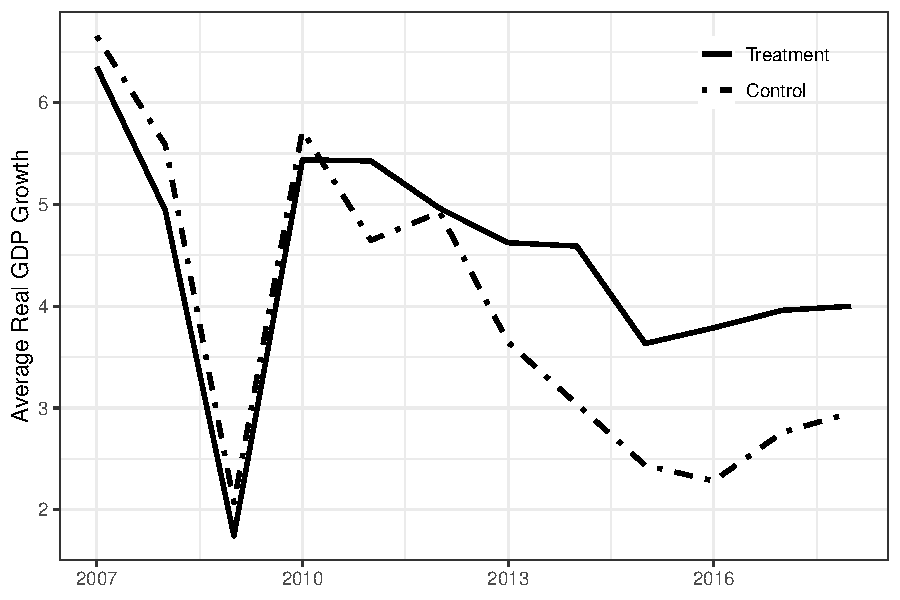
\includegraphics[width=0.70\columnwidth]{figures/rgdpg/rgdpg}
\caption{{Average Real GDP Growth (Treatment vs Control Group). Data source: World
Bank. The Treatment Group includes the countries that have experienced
BRI-induced investment shocks. The Control Group consists of countries
of similar levels of development as those in the Treatment Group but
never experienced investment shock.~
{\label{847236}}%
}}
\end{center}
\end{figure}

\par\null

\subsection{Staggered
Difference-in-Difference}\label{staggered-difference-in-difference}

With the matched sample, I exploit the variation resulting from the
different timing of the investment shock induced by the BRI to estimate
the effects of such investment on a country's economic growth. Although
certain country-specific characteristics might be associated with the
probability of receiving BRI investment, there is also a strong random
component due to the policy shock. This motivates a staggered
difference-in-difference approach in which the timing of the treatment
varies by country ~\hyperref[csl:18]{(Goodman-Bacon 2018}; \hyperref[csl:19]{Callaway and Sant'Anna 2019)}. Thus the composition of the
treatment and control groups evolves over time. In any specific year in
the sample, the control group consists of both the countries that would
never be treated and the countries that were yet to be treated.

Specifically, I estimate the following model to identify the treatment
effect:

\begin{equation}
\label{eq:baseline}
\log(\textrm{GDP})_{c,t} = \beta\textrm{PostBRI}_{c,t} + \gamma_c + \delta_t + \mathbf{Z}_c\delta_t + \gamma_c t + \mathbf{X}_{c,t} + \epsilon_{c,t}
\end{equation}

$\textrm{GDP}_{c,t}$ is the real GDP (in constant US dollar) for country $c$ and year $t$.
$\textrm{PostBRI}_{c,t}$ is the treatment indicator that equals to one if country $c$ has experienced BRI-induced investment shock no later than year $t$.
$\gamma_c$ is a vector of country fixed effects.
$\delta_t$ is a vector of year fixed effects.
$\mathbf{Z}_c$ is a vector of dummy variables encoding whether a country is landlocked, resource-rich, or heavily indebted. $\mathbf{Z}_c$ is interacted with $\delta_t$ to control for differential year fixed effects for different situated countries.
$\gamma_c t $ denote the interaction terms between country fixed effects and a continuous time variable. This allows different economic trends for each individual country.
Finally, $\mathbf{X}_{c,t}$, a vector of time-variant variables that could possibly influence economic outcomes are also controlled, including urbanization, human capital accumulation, international aid and so on.



\section{\texorpdfstring{{Empirical
Results}}{Empirical Results}}

{\label{411455}}

\subsection{Effect on Economic Growth}

{\label{783625}}

Table~{\ref{tab:baseline}}~presents the results of the
OLS estimation of Specification~{\ref{eq:baseline}} .
The first column reports the baseline results in which only ~country and
year fixed effects are controlled. The second and third columns include
interactions between various country profile dummies and year fixed
effects. These country profile dummies include whether a country is a
Least Developed Country (LDC), landlocked, a fuel exporter (a proxy for
resource endowment), or geographically located on the belt and road. The
forth column further includes the interactions between country fixed
effects and the time variable to further allow different economic trends
for each individual country.~\selectlanguage{english}
\begin{table}[!htbp] \centering
  \caption{{The Impact of BRI investment on Economic Growth}}
  \label{tab:baseline}
\begin{tabular}{@{\extracolsep{5pt}}lcccc}
\\[-1.8ex]\hline
\hline \\[-1.8ex]
\\[-1.8ex] & (1) & (2) & (3) & (4)\\
\hline \\[-1.8ex]
 PostBRI & 0.052$^{***}$ & 0.053$^{***}$ & 0.053$^{***}$ & 0.019$^{***}$ \\
  & (0.011) & (0.010) & (0.011) & (0.007) \\
  & & & & \\

Country FE & Yes & Yes & Yes & Yes \\
Year FE & Yes & Yes & Yes & Yes \\
LDC $\times$ FE & No & Yes & Yes & Yes \\
Landlocked $\times$ FE & No & Yes & Yes & Yes \\
Fuel $\times$ FE & No & No & Yes & Yes \\
Belt\&Road $\times$ FE & No & No & Yes & Yes \\
Country FE $\times$ $t$ & No & No & No & Yes \\

\hline \\[-1.8ex]
Observations & 785 & 785 & 785 & 785 \\
Adjusted R$^{2}$ & 0.997 & 0.997 & 0.997 & 0.999 \\
\hline
\hline \\[-1.8ex]
\end{tabular}

\begin{flushleft}
\textit{Note:} This table reports the difference-in-difference
estimation of the impact of BRI investment on economic growth.
Dependent variable is the natural log of real GDP.
Coefficients are interpretated as the percentage change in the  real GDP of the relevant countries due to the BRI-induced investment shock.
Robust standard errors are in parentheses.
$^{*}$p$<$0.1; $^{**}$p$<$0.05; $^{***}$p$<$0.01
\end{flushleft}

\end{table}

The results presented in Table~{\ref{tab:baseline}}~is
striking. The BRI-induced investment is estimated to boost the recipient
countries' real GDP by more than 5\%. This estimation is unscathed even
taking into consideration of the economic backwardness, natural resource
endowment and geographical location. Incorporating different time trends
for each individual country (the forth column) reduces the magnitude of
the coefficient to around 2\%, but the treatment effect is still sizable
and statistically significant.

To address the concern of possible time-variant factors that could bias
the result. Table~{\ref{tab:timevar}}~reports the
results after controlling various time-variant factors the could
possibly influence economic outcomes. These factors include the
percentage of urban population to total population as a proxy for
urbanization, school life expectancy (primary to tertiary) as a proxy
for human capital, net Official Development Aid (ODA) received as a
measure of international aid effort, and government expenditure as a
proxy for government capability.~\selectlanguage{english}
\begin{table}[!htbp] \centering
  \caption{{The Impact of BRI Investment on Economic Growth}}
  \label{tab:timevar}
\begin{tabular}{@{\extracolsep{5pt}}lcccc}
\\[-1.8ex]\hline
\hline \\[-1.8ex]
\\[-1.8ex] & (1) & (2) & (3) & (4)\\
\hline \\[-1.8ex]
 PostBRI & 0.054$^{***}$ & 0.030$^{**}$ & 0.035$^{***}$ & 0.042$^{***}$ \\
  & (0.011) & (0.012) & (0.013) & (0.013) \\
  & & & & \\
 Urban Population (\%) & $-$0.009$^{**}$ & 0.003 & $-$0.0001 & $-$0.001 \\
  & (0.005) & (0.005) & (0.005) & (0.006) \\
  & & & & \\
 School Life Expectancy &  & 0.023$^{***}$ & 0.022$^{***}$ & 0.027$^{***}$ \\
  &  & (0.008) & (0.008) & (0.008) \\
  & & & & \\
 Log Net ODA &  &  & 0.001 & $-$0.013$^{*}$ \\
  &  &  & (0.007) & (0.007) \\
  & & & & \\
 Log Government Expenditure &  &  &  & 0.160$^{***}$ \\
  &  &  &  & (0.029) \\
  & & & & \\
\hline \\[-1.8ex]
Country FE & Yes & Yes & Yes & Yes \\
Year FE & Yes & Yes & Yes & Yes \\
Observations & 785 & 384 & 362 & 223 \\
Adjusted R$^{2}$ & 0.997 & 0.999 & 0.999 & 0.999 \\
\hline
\hline \\[-1.8ex]
\textit{Note:}  & \multicolumn{4}{r}{$^{*}$p$<$0.1; $^{**}$p$<$0.05; $^{***}$p$<$0.01} \\
\end{tabular}

\end{table}

Though some of these factors do have a significant influence over the
economic outcome, they do not undermine the effect of BRI investment.
The estimated treatment effects ranges from 3\% to 5\%, all with
statistical significance. But the results reported in Table
{\ref{tab:timevar}}~should be interpreted with a
caveat. ~Due to the data availability issue, including these factors
greatly reduce the sample size. Many countries with missing data are
among those least developed countries. Excluding these countries from
the sample could possibly induce biases to the estimation.~

\par\null

\subsection{Effect by Sectors}

{\label{680783}}

To shed some lights on the mechanism of how the BRI investment boosts
the economic growth of relevant countries, I estimate the effects of BRI
investment on host countries' agriculture, industry and international
trade. The results are reported in
Table~{\ref{tab:industry}}. Column (1)-(3) reports the
treatment effects on agriculture value-added, industry value-added, and
trade volume (import plus export) respectively. ~A full list of fixed
effects (country and year fixed effects together with country profile
dummies interacted with year fixed effects) are controlled throughout.~\selectlanguage{english}
\begin{table}[!htbp] \centering
  \caption{{The Effect of BRI investment on Agriculture, Industry, and Trade}}
  \label{tab:industry}
\begin{tabular}{@{\extracolsep{5pt}}lccc}
\\[-1.8ex]\hline
\hline \\[-1.8ex]
 & Agriculture V.A. & Industry V.A. & Trade Vol. \\
\\[-1.8ex] & (1) & (2) & (3)\\
\hline \\[-1.8ex]
 PostBRI & 0.054$^{***}$ & 0.132$^{***}$ & $-$0.039 \\
  & (0.020) & (0.026) & (0.033) \\
  & & & \\

Country FE & Yes & Yes & Yes \\
Year FE & Yes & Yes & Yes \\
Country Profile $\times$ FE & Yes & Yes & Yes \\

\hline \\[-1.8ex]
Observations & 776 & 776 & 754 \\
Adjusted R$^{2}$ & 0.991 & 0.986 & 0.967 \\
\hline
\hline \\[-1.8ex]
\textit{Note:}  & \multicolumn{3}{r}{$^{*}$p$<$0.1; $^{**}$p$<$0.05; $^{***}$p$<$0.01} \\
\end{tabular}
\end{table}

Table~{\ref{tab:industry}}~shows that the BRI
investment increase the recipient countries's agriculture value-added by
5\%, and industry value-added by a remarkable 13\%. This indicates that
the BRI program greatly promotes the industrialization of its members.
The effect on trade volume is, however, slightly negative and
imprecisely estimated. This is somewhat surprising because many believe
that the BRI is intended to promote trade with China.~

\par\null

\subsection{Effect by Region and Income
Group}

{\label{689555}}

I further disaggregate the main results by region and income group by
interacting the treatment variable with region and income-group dummies.
Table~{\ref{tab:region}}~reports the results. It shows
that the BRI investment has strong positive effect on economic growth
for countries in South Asia, East Asia , and Sub-Saharan Africa, and
countries in low income or lower middle income group. The effects are
not pronounced, or even negative, for countries located in Europe or
Middle East, and countries with upper middle income. These results are
mostly expected, as lower income countries are more likely to experience
higher growth rate when exposed to BRI investment. But there is also a
caveat associated with these results: as the propensity score matching
is conducted over the entire sample, not within specific region or
income group, these coefficients might not be as sensible as the
coefficients estimated over the entire sample.\selectlanguage{english}
\begin{table}[!htbp] \centering
  \caption{{Effect of BRI investment by Region and Income Group}}
  \label{tab:region}
\begin{tabular}{@{\extracolsep{5pt}}lcc}
\\[-1.8ex]\hline
\hline \\[-1.8ex]
\\[-1.8ex] & (1) & (2)\\
\hline \\[-1.8ex]
 PostBRI & 0.072$^{***}$ & 0.086$^{***}$ \\
  & (0.013) & (0.011) \\
  & & \\
 South Asia & 0.008 &  \\
  & (0.017) &  \\
  & & \\
 Europe \& Central Asia & $-$0.121$^{***}$ &  \\
  & (0.018) &  \\
  & & \\
 Middle East \& North Africa & $-$0.097$^{***}$ &  \\
  & (0.017) &  \\
  & & \\
 East Asia \& Pacific & 0.039$^{**}$ &  \\
  & (0.017) &  \\
  & & \\
 Sub-Saharan Africa & $-$0.011 &  \\
  & (0.017) &  \\
  & & \\
 Latin America \& Caribbean &  &  \\
  & - &  \\
  & & \\


 Low income &  & 0.010 \\
  &  & (0.018) \\
  & & \\
 Upper middle income &  & $-$0.141$^{***}$ \\
  &  & (0.019) \\
  & & \\
 Lower middle income &  &  \\
  &  & - \\
  & & \\

Country FE & Yes & Yes \\
Year FE & Yes & Yes \\

\hline \\[-1.8ex]

Observations & 785 & 785 \\
Adjusted R$^{2}$ & 0.997 & 0.998 \\
\hline
\hline \\[-1.8ex]
\textit{Note:}  & \multicolumn{2}{r}{$^{*}$p$<$0.1; $^{**}$p$<$0.05; $^{***}$p$<$0.01} \\
\end{tabular}
\end{table}

\par\null

\section{Robustness Checks}

{\label{351972}}

\subsection{Sensitivity Test}

{\label{254092}}

I conduct various sensitivity tests to test the robustness of the
baseline results. First, I test the sensitivity of the baseline results
to the sample chosen by randomly omitting 10 countries in the sample and
re-estimate the treatment effect. I run the test 100 times and the
distribution of the estimated treatment effect is plotted in
Figure~{\ref{339676}}. The distribution is roughly
normal-distributed around 5.2\%. This confirms the baseline results
reported in Table~{\ref{tab:baseline}}~are not driven
by particular countries in the sample. The distribution of the upper and
lower bonds of the confidence intervals (shadow curves in the graph)
confirms that the treatment effects are significantly different from
zero whatever the sample chosen.~\selectlanguage{english}
\begin{figure}[H]
\begin{center}
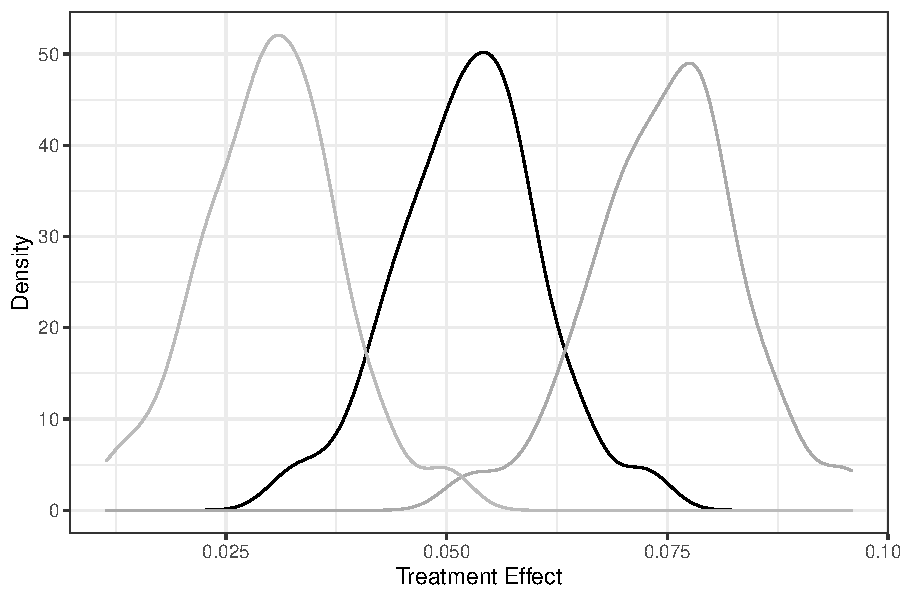
\includegraphics[width=0.70\columnwidth]{figures/sstest1/sstest1}
\caption{{Distribution of the Estimated Treatment Effects. Source: author's
estimation. This figure plots the distribution of the estimated
treatment effects by repeating the baseline regression 100 times, each
time with 10 countries removed from the sample randomly. The shadow
curves are the distribution of the lower and upper bounds of the 95\%
confidence intervals. ~~
{\label{339676}}%
}}
\end{center}
\end{figure}

Second, I test the sensitivity of the baseline results to different
criteria of treatment identification by raising or lowering the
thresholds of identifying an investment shock. Details of this test are
in Appendix~{\ref{224476}}. The conclusion is, although
different criteria yield different samples, it does not undermine the
treatment effect. The magnitudes of the estimated coefficients may vary
due to different criteria, the treatment effects are always
significantly different from zero. ~

Third, the baseline results assume equal weights for every observation.
It might make more sense if countries are weighted by their economic
size. I rerun the baseline regression with countries weighted by their
economic size. I find similar results as the baseline.

\par\null

\subsection{Timing~}

{\label{178154}}

Timing evidence is crucial for a causal interpretation of the results.
It is of particular interest that the economic growth postdated the BRI
investment, not the other way around. To test this assumption, I include
leading dummies in the regression, coding dummies for whether a country
will experience a BRI investment shock in 2-5 years.
Table~{\ref{tab:timing}}~reports the results. The
coefficients of these leading dummies are very small and imprecisely
estimated. This confirms that the economic growth indeed happened after
the BRI investment, not predated it.
Table~{\ref{tab:timing}}~also serves as a double-check
of the parallel assumption that there is no difference in economic
growth between the treatment and control group before the treatment. ~\selectlanguage{english}
\begin{table}[!htbp] \centering
  \caption{{Timing of Economic Growth to BRI Investment}}
  \label{tab:timing}
\begin{tabular}{@{\extracolsep{5pt}}lcccc}
\\[-1.8ex]\hline
\hline \\[-1.8ex]
\\[-1.8ex] & (1) & (2) & (3) & (4)\\
\hline \\[-1.8ex]
 2 years before treatment & $-$0.017$^{*}$ &  &  &  \\
  & (0.010) &  &  &  \\
  & & & & \\
 3 years before treatment &  & $-$0.013 &  &  \\
  &  & (0.011) &  &  \\
  & & & & \\
 4 years before treatment &  &  & 0.0002 &  \\
  &  &  & (0.015) &  \\
  & & & & \\
 5 years before treatment &  &  &  & 0.008 \\
  &  &  &  & (0.016) \\
  & & & & \\

Country FE & Yes & Yes & Yes & Yes \\
Year FE & Yes & Yes & Yes & Yes \\

\hline \\[-1.8ex]
Observations & 399 & 399 & 399 & 399 \\
Adjusted R$^{2}$ & 0.998 & 0.998 & 0.998 & 0.998 \\
\hline
\hline \\[-1.8ex]
\textit{Note:}  & \multicolumn{4}{r}{$^{*}$p$<$0.1; $^{**}$p$<$0.05; $^{***}$p$<$0.01} \\
\end{tabular}
\end{table}

\subsection{Dynamic Effect}

{\label{817671}}

To gauge deeper into how the BRI influences economic outcomes, I explore
the dynamic effects of the BRI investment by estimating the following
model:

\begin{equation}
\label{eq:dynamic}
\log(\textrm{GDP})_{c,t} = \sum_{\tau \in \{-5,\dots, 5\}} \beta_{\tau} \textrm{PostBRI}_{c,\tau} + \gamma_c + \delta_t + \mathbf{Z}_c\delta_t + \gamma_c t  + \epsilon_{c,t}
\end{equation}

$\textrm{PostBRI}_{c,\tau}$ is a set of dummies that equal to $1$ if it has been $\tau$ years after the first BRI investment shock, where $\tau\in\{t \in \mathbb{Z}| -5 \leq t \leq 5 \}$.
The sequence of $\{ \beta_{\tau} \}$ speak for the dynamic effects of the BRI investment over time.


Note that this automatically discards the countries that received no
treatment at all. The OLS estimation of the dynamic effect is presented
in Figure~{\ref{685807}}, with a full set of fixed
effects controlled. The estimated coefficients are small and imprecise
until 2 years after the investment shock, and gradually magnifies as
years pass by. This result is aligned with the common sense that it
takes time for an investment to take effect on economic outcomes.~\selectlanguage{english}
\begin{figure}[H]
\begin{center}
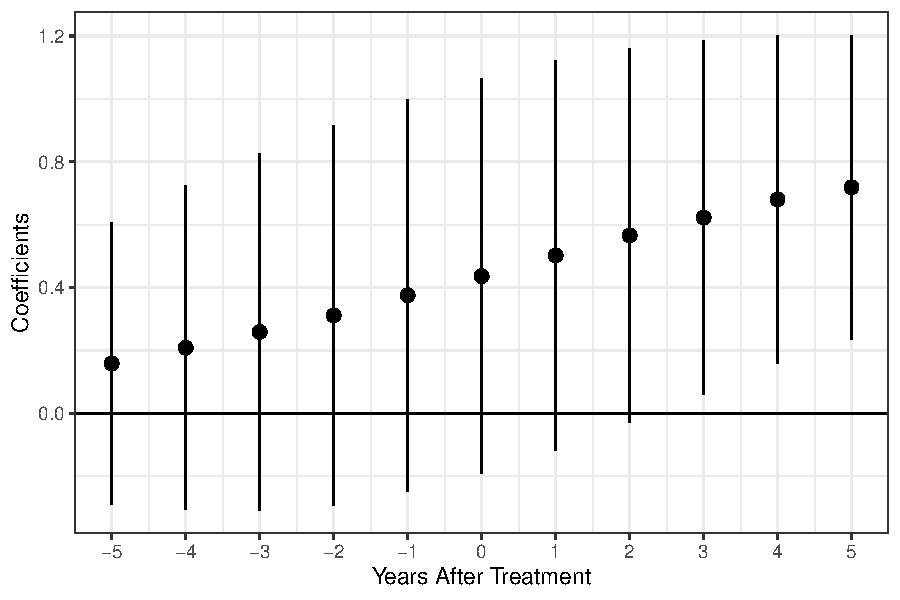
\includegraphics[width=0.70\columnwidth]{figures/dyncoefs/dyncoefs}
\caption{{Dynamic Effects of the BRI Investment. Bars represent 95\% CI.
{\label{685807}}%
}}
\end{center}
\end{figure}

\subsection{Selection Concerns}

{\label{310737}}

It is a natural concern that the BRI investment is subject to selection.
Rather than BRI investment causes economic growth, it is China picks the
countries with growth potential that drives the results. China is also
criticized by some as a neocolonial power as China has been investing
heavily in resource-rich countries. Though the results reported in
Table~{\ref{tab:baseline}}~controlling for natural
resource endowment and other country profiles should somewhat mitigate
the concern, it could be argued that there are other aspects of growth
potential that are not captured.

To address this concern, I make use of the IMF World Economic Outlook
(WEO). The WEO is IMF's biannual report which includes IMF economists'
forecast for each country's GDP for the next a few years. The WEO is
regarded by many as the best economic forecast available and it takes
into account a variety of factors that could possibly influence economic
outcomes. The difference between the actual GDP growth and the IMF
forecasted growth can be interpreted as a shock, in the sense that it
reflects the deviation of the economy from its expected courses as
estimated by some of the best experts in the world. I regress this
difference on the BRI investment. The estimated coefficient speaks for
the positive or negative shocks that the BRI brings about to the
economy. This estimation is, to the largest possible extent, freed of
selection concerns because IMF's forecasts should have taken into
account the growth potential of each country to the best of the
knowledge available.\selectlanguage{english}
\begin{table}[!htbp] \centering
  \caption{{BRI Investment and Economic Shocks}}
  \label{tab:shocks}
\begin{tabular}{@{\extracolsep{5pt}}lccc}
\\[-1.8ex]\hline
\hline \\[-1.8ex]

 & (1) & (2) & (3)\\
\hline \\[-1.8ex]

 PostBRI & 0.075$^{***}$ & 0.081$^{***}$ & 0.091$^{***}$ \\
  & (0.026) & (0.026) & (0.025) \\
  & & & \\

Country FE & Yes & Yes & Yes \\
Year FE & Yes & Yes & Yes \\
LDC $\times$ FE & No & Yes & Yes \\
Landlocked $\times$ FE & No & Yes & Yes \\
Fuel $\times$ FE & No & No & Yes \\
Belt\&Road $\times$ FE & No & No & Yes \\

\hline \\[-1.8ex]
Observations & 544 & 544 & 544 \\
Adjusted R$^{2}$ & 0.748 & 0.746 & 0.764 \\
\hline
\hline \\[-1.8ex]

\end{tabular}

\begin{flushleft}
\textit{Note:}
The dependent variable is the natural log difference between
actual GDP and IMF forecasted GDP.
The coefficients are interpretated as the percentage-point difference between the treated and untreated countries regarding how much their actual GDP deviates from IMF's forecast.
Robust standard errors are in parentheses.
$^{*}$p$<$0.1; $^{**}$p$<$0.05; $^{***}$p$<$0.01
\end{flushleft}

\end{table}

Table~{\ref{tab:shocks}}~reports the estimation of
economic shocks that the BRI brings about. I use IMF's World Economic
Outlook in April 2013 which includes forecasted GDP for each country up
to 2018. I replicate the regressions in
Table~{\ref{tab:baseline}} but with the log difference
between the actual GDP and the IMF forecasted GDP as the dependent
variable. The result shows that the actual GDP of the treated countries
positively deviate from the IMF's forecast by around 8 percentage point
more than the untreated countries. This~{confirms that the BRI
investment contributes a significant positive shock to the recipient
economies.~~}

\par\null

\section{Conclusion}

{\label{322007}}

Since the announcement of the Belt and Road Initiative in 2013, China's
investments in the belt and road countries increased dramatically. This
paper estimates the impact of the BRI investment on the relevant
countries' economic outcomes by a staggered difference-in-difference
method. The study finds that the BRI investments significantly boost the
treated countries' real GDP by 5\% on average compared to untreated
countries. The effects are more pronounced for low income countries in
South Asia, East Asia, Sub-Saharan Africa. Evidence also suggests that
the BRI program helps some developing countries to industrialize. These
results are robust against various sensitivity tests and are not biased
by reverse causality or selection issues.~

However, these results should be interpreted with a caveat. This study
does not address the debt burdens that the massive investments impose on
some countries. Whether the accumulating debt would cause~financial
stress or even financial instability is still unknown at the present.
Therefore, the cost and benefit of such an ambitious program remains an
open question. Besides, the GDP should not be regarded as the sole
measure of wellbeing. To figure out what this massive program brings to
each of its member countries requires inclusive studies of every
economic and social aspects. This, of course, goes far beyond the scope
of this paper, and is therefore left for future studies.~

\par\null

\section{Appendix}
\label{sec:appendix}
\beginsupplement

\subsection{Criteria of treatment}

{\label{639717}}

A treatment is identified if a country recieves significant more FDI
from China after joining the BRI. Figure~{\ref{554014}}
demostrates the idea. Vietnam is not considered treated, because there
is no significiant increase in investment from China after 2013. While
Pakistan is identified as treated starting from 2014 when the investment
from China exploded. For countries that never receive investments from
China prior to BRI and starts to receive investment thereafter, they are
regarded as treated only if the investment flows are sizable enough. For
example, Namibia is not regarded as treated even if it joind the BRI and
started to receive Chinese investments, because the amount of
investments is too small to be considered seriously. While Uganda is
condered treated as the investments it received are sizable enough.\selectlanguage{english}
\begin{figure}[H]
\begin{center}
\includegraphics[width=0.70\columnwidth]{figures/Rplot04/Rplot04}
\caption{{China's Investments in some Countries
{\label{554014}}%
}}
\end{center}
\end{figure}

Therefore, there are two critical thresholds for a country to be
identified as treated: (i) the amount of annual investments it receives
from China has to pass an entry bar, say~\(\theta\); (ii) if it
has received investments from China before the BRI, the investment flows
after the BRI has to be at least~\(\kappa\) times greater than
the maximal investments preexited in~\(\tau\) years.~These
thresholds for identifying a treatment is imposed to make sure that it
is identifying an investment shock induced by the BRI, not regular flows
of investments that would have happened even in natural courses.~

\subsection{Sensitivity test of the
criteria}

{\label{224476}}

I test the sensitity of the baseline results to the criteria of
identifying a treatment by raising or lowering the thresholds mentioned
above. First, I keep at constant~\(\kappa=2\)
and~\(\tau=3\), and impose different values
to~\(\theta\). The estimated treatment effects for
different~\(\theta\) are plotted in
Figure~{\ref{813720}}. It shows that the treatment
effects estimated tend to be larger for higher thresholds of investment
quantities. This is expected as more sizable investments tend to have
larger impact on economic outcomes.~\selectlanguage{english}
\begin{figure}[H]
\begin{center}
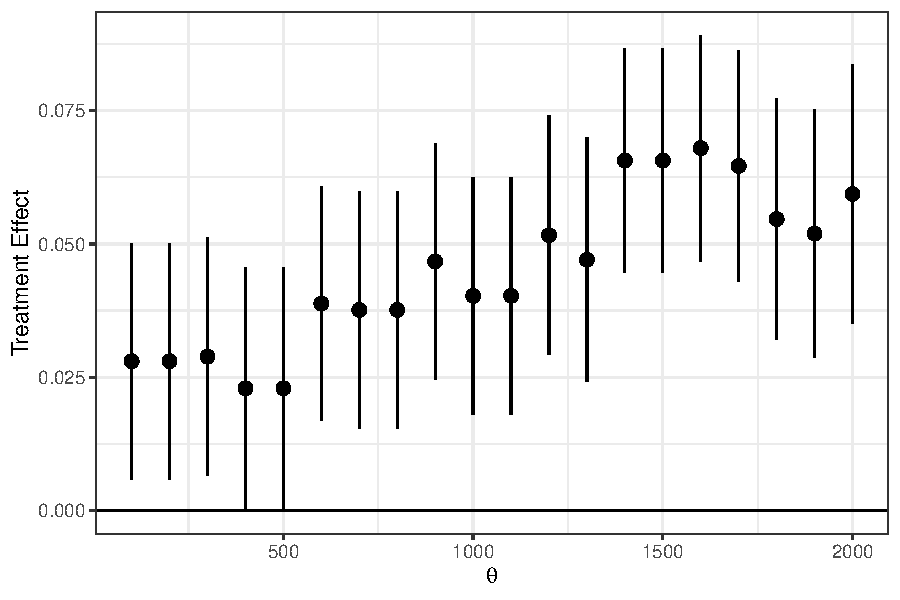
\includegraphics[width=0.70\columnwidth]{figures/sstest3/sstest3}
\caption{{Estimated Treatment Effects for Different Levels of~\(\theta\)
{\label{813720}}%
}}
\end{center}
\end{figure}

Second, I keep~\(\theta=800\) and~\(\tau=3\), raise and
lower the value of~\(\kappa\).
Figure~{\ref{688913}} plots how the treatement effects
estimated vary along with different values of~\(\kappa\). The
results are also compatible with usual expectation -- the higher the
thresholds, the larger the estimated treatment effects. But it seems
that raising the thresholds too high tends to have the opposite effect,
probably because it reduces the sample size too much.~\selectlanguage{english}
\begin{figure}[H]
\begin{center}
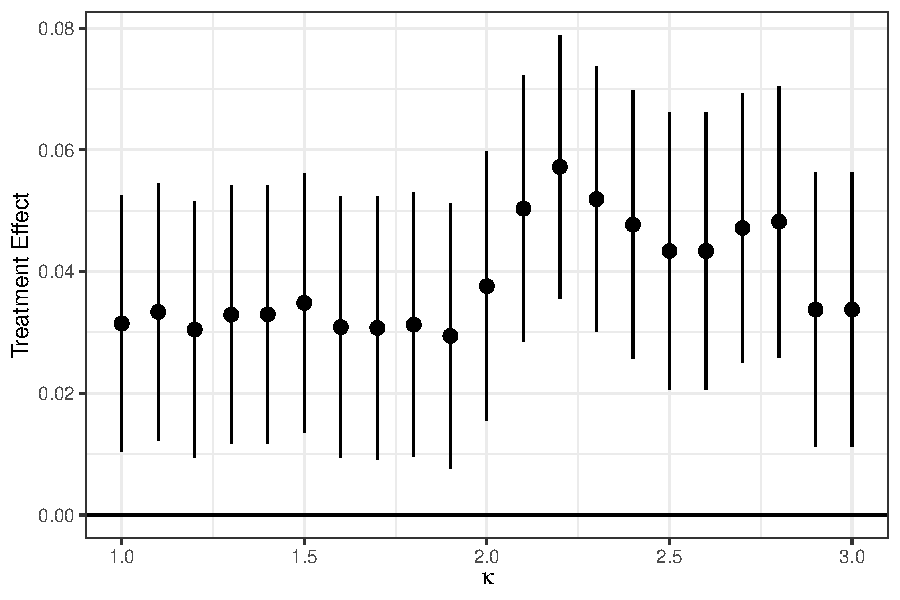
\includegraphics[width=0.70\columnwidth]{figures/sstest2/sstest2}
\caption{{Estimated Treatment Effects for Different Levels of~\(\kappa\)
{\label{688913}}%
}}
\end{center}
\end{figure}

The sample used in the main body of this poper employs a flexible set of
thresholds for the most plausible identification of investment shocks
for each country.~

\subsection{List of treated and untreated
countries}

{\label{203131}}\selectlanguage{english}
\begin{table}[!htbp] \centering   \caption{{Countries in Treatment and Control Groups}}   \label{tab:appendix} \begin{tabular}{@{\extracolsep{5pt}} llccc} \\[-1.8ex]\hline \hline \\[-1.8ex]  & Country Name & ISO3 Code & Group & Treated Year \\ \hline \\[-1.8ex] 1 & Azerbaijan & AZE & Treatment & $2018$ \\ 2 & Bangladesh & BGD & Treatment & $2013$ \\ 3 & Bolivia (Plurinational State of) & BOL & Treatment & $2014$ \\ 4 & Cambodia & KHM & Treatment & $2017$ \\ 5 & Cameroon & CMR & Treatment & $2015$ \\ 6 & Chad & TCD & Treatment & $2011$ \\ 7 & Congo & COG & Treatment & $2014$ \\ 8 & C\selectlanguage{ngerman}ôte d\selectlanguage{english}'Ivoire & CIV & Treatment & $2013$ \\ 9 & Egypt & EGY & Treatment & $2015$ \\ 10 & Equatorial Guinea & GNQ & Treatment & $2013$ \\ 11 & Ethiopia & ETH & Treatment & $2013$ \\ 12 & Ghana & GHA & Treatment & $2012$ \\ 13 & Guinea & GIN & Treatment & $2015$ \\ 14 & Indonesia & IDN & Treatment & $2015$ \\ 15 & Iran (Islamic Republic of) & IRN & Treatment & $2016$ \\ 16 & Jordan & JOR & Treatment & $2013$ \\ 17 & Kazakhstan & KAZ & Treatment & $2017$ \\ 18 & Kenya & KEN & Treatment & $2012$ \\ 19 & Kyrgyzstan & KGZ & Treatment & $2014$ \\ 20 & Lao People's Democratic Republic & LAO & Treatment & $2015$ \\ 21 & Madagascar & MDG & Treatment & $2015$ \\ 22 & Malaysia & MYS & Treatment & $2012$ \\ 23 & Mali & MLI & Treatment & $2015$ \\ 24 & Mongolia & MNG & Treatment & $2015$ \\ 25 & Montenegro & MNE & Treatment & $2014$ \\ 26 & Mozambique & MOZ & Treatment & $2012$ \\ 27 & Nepal & NPL & Treatment & $2018$ \\ 28 & Nigeria & NGA & Treatment & $2013$ \\ 29 & Pakistan & PAK & Treatment & $2014$ \\ 30 & Papua New Guinea & PNG & Treatment & $2017$ \\ 31 & Philippines & PHL & Treatment & $2014$ \\ 32 & Russian Federation & RUS & Treatment & $2014$ \\ 33 & Senegal & SEN & Treatment & $2015$ \\ 34 & Serbia & SRB & Treatment & $2017$ \\ 35 & Sri Lanka & LKA & Treatment & $2013$ \\ 36 & Thailand & THA & Treatment & $2016$ \\ 37 & Uganda & UGA & Treatment & $2013$ \\ 38 & United Republic of Tanzania & TZA & Treatment & $2013$ \\ 39 & Zambia & ZMB & Treatment & $2015$ \\ 40 & Zimbabwe & ZWE & Treatment & $2015$ \\ 41 & Afghanistan & AFG & Control & $$ \\ 42 & Algeria & DZA & Control & $$ \\ 43 & Angola & AGO & Control & $$ \\ 44 & Belarus & BLR & Control & $$ \\ 45 & Benin & BEN & Control & $$ \\ 46 & Brazil & BRA & Control & $$ \\ 47 & Burkina Faso & BFA & Control & $$ \\ 48 & Burundi & BDI & Control & $$ \\ 49 & Central African Republic & CAF & Control & $$ \\ 50 & Colombia & COL & Control & $$ \\ 51 & Dominican Republic & DOM & Control & $$ \\ 52 & Ecuador & ECU & Control & $$ \\ 53 & El Salvador & SLV & Control & $$ \\ 54 & Guatemala & GTM & Control & $$ \\ 55 & Haiti & HTI & Control & $$ \\ 56 & Iraq & IRQ & Control & $$ \\ 57 & Lesotho & LSO & Control & $$ \\ 58 & Liberia & LBR & Control & $$ \\ 59 & Malawi & MWI & Control & $$ \\ 60 & Mauritania & MRT & Control & $$ \\ 61 & Mexico & MEX & Control & $$ \\ 62 & Morocco & MAR & Control & $$ \\ 63 & Myanmar & MMR & Control & $$ \\ 64 & Niger & NER & Control & $$ \\ 65 & Paraguay & PRY & Control & $$ \\ 66 & Peru & PER & Control & $$ \\ 67 & Rwanda & RWA & Control & $$ \\ 68 & Sierra Leone & SLE & Control & $$ \\ 69 & Sudan & SDN & Control & $$ \\ 70 & Tajikistan & TJK & Control & $$ \\ 71 & Timor-Leste & TLS & Control & $$ \\ 72 & Togo & TGO & Control & $$ \\ 73 & Turkey & TUR & Control & $$ \\ 74 & Turkmenistan & TKM & Control & $$ \\ 75 & Ukraine & UKR & Control & $$ \\ 76 & Uzbekistan & UZB & Control & $$ \\ 77 & Venezuela (Bolivarian Republic of) & VEN & Control & $$ \\ 78 & Viet Nam & VNM & Control & $$ \\ 79 & Yemen & YEM & Control & $$ \\ \hline \\[-1.8ex] \end{tabular} \end{table}

\selectlanguage{english}
\FloatBarrier
\section*{References}\sloppy
\phantomsection
\label{csl:1}Campbell, Charlie. 2017. ``{What to Know About China's Belt and Road Initiative Summit}''. \textit{Times}. \url{https://time.com/4776845/china-xi-jinping-belt-road-initiative-obor/.}

\phantomsection
\label{csl:2}Xinhua. 2015. ``{Chronology of China’s Belt and Road Initiative}''. \textit{The State Council of the People's Republic of China}. \url{http://english.www.gov.cn/news/top_news/2015/04/20/content_281475092566326.htm.}

\phantomsection
\label{csl:3}———. 2015. ``{China Unveils Action Plan on Belt and Road Initiative}''. \textit{The State Council of the People's Republic of China}. \url{http://english.www.gov.cn/news/top_news/2015/03/28/content_281475079055789.htm.}

\phantomsection
\label{csl:4}———. 2019. ``{China Focus: Belt and Road Initiative Makes Solid Progress, Embraces Brighter Future}''. \textit{XinhuaNET}. \url{http://www.xinhuanet.com/english/2019-04/23/c_137999264.htm.}

\phantomsection
\label{csl:5}Scobell, Andrew, Bonny Lin, Howard J Shatz, Larry Hanauer, Michael Johnson, Michael S Chase, Astrid Stuth Cevallos, et al. 2018. \textit{{At the Dawn of Belt and Road: China in the Developing World}}. Rand Corporation.

\phantomsection
\label{csl:6}Huang, Yiping. 2016. ``{Understanding China{\Textquotesingle}s Belt {\&} Road Initiative: Motivation Framework and Assessment}''. \textit{China Economic Review} 40 (September): 314–21. \url{https://doi.org/10.1016/j.chieco.2016.07.007.}

\phantomsection
\label{csl:7}Yu, Hong. 2016. ``{Motivation behind China's `One Belt One Road' Initiatives and Establishment of the Asian Infrastructure Investment Bank}''. \textit{Journal of Contemporary China} 26 (105): 353–68. \url{https://doi.org/10.1080/10670564.2016.1245894.}

\phantomsection
\label{csl:8}Du, Julan, and Yifei Zhang. 2018. ``{Does One Belt One Road Initiative Promote Chinese Overseas Direct Investment?}''. \textit{China Economic Review} 47 (February): 189–205. \url{https://doi.org/10.1016/j.chieco.2017.05.010.}

\phantomsection
\label{csl:9}Chellaney, Brahma. 2017. ``{China’s Debt-Trap Diplomacy}''. \textit{Project Syndicate}. \url{https://www.project-syndicate.org/commentary/china-one-belt-one-road-loans-debt-by-brahma-chellaney-2017-01.}

\phantomsection
\label{csl:10}Anderlini, Jamil. 2018. ``{China Is at Risk of Becoming a Colonialist Power}''. \textit{Financial Times}. \url{https://www.ft.com/content/186743b8-bb25-11e8-94b2-17176fbf93f5.}

\phantomsection
\label{csl:11}D{\'{e}}murger, Sylvie. 2001. ``{Infrastructure Development and Economic Growth: An Explanation for Regional Disparities in China?}''. \textit{Journal of Comparative Economics} 29 (1): 95–117. \url{https://doi.org/10.1006/jcec.2000.1693.}

\phantomsection
\label{csl:12}Fan, Shenggen, and Xiaobo Zhang. 2004. ``{Infrastructure and Regional Economic Development in Rural China}''. \textit{China Economic Review} 15 (2): 203–14. \url{https://doi.org/10.1016/j.chieco.2004.03.001.}

\phantomsection
\label{csl:13}Banerjee, Abhijit, Esther Duflo, and Nancy Qian. 2012. ``{On the Road: Access to Transportation Infrastructure and Economic Growth in China}''. National Bureau of Economic Research. \url{https://doi.org/10.3386/w17897.}

\phantomsection
\label{csl:14}Huang, Yasheng. 2008. \textit{{Capitalism with Chinese Characteristics}}. Cambridge University Press. \url{https://doi.org/10.1017/cbo9780511754210.}

\phantomsection
\label{csl:15}Ansar, Atif, Bent Flyvbjerg, Alexander Budzier, and Daniel Lunn. 2016. ``{Does Infrastructure Investment Lead to Economic Growth or Economic Fragility? Evidence from China}''. \textit{Oxford Review of Economic Policy} 32 (3): 360–90. \url{https://doi.org/10.1093/oxrep/grw022.}

\phantomsection
\label{csl:16}Yu, Linhui, Dan Zhao, Haixia Niu, and Futao Lu. 2020. ``{Does the Belt and Road Initiative Expand China{\Textquotesingle}s Export Potential to Countries along the Belt and Road?}''. \textit{China Economic Review} 60 (April): 101419. \url{https://doi.org/10.1016/j.chieco.2020.101419.}

\phantomsection
\label{csl:17}Soyres, Fran{\c{c}}ois de, Alen Mulabdic, and Michele Ruta. 2020. ``{Common Transport Infrastructure: A Quantitative Model and Estimates from the Belt and Road Initiative}''. \textit{Journal of Development Economics} 143 (March): 102415. \url{https://doi.org/10.1016/j.jdeveco.2019.102415.}

\phantomsection
\label{csl:18}Goodman-Bacon, Andrew. 2018. ``{Difference-in-Differences with Variation in Treatment Timing}''. National Bureau of Economic Research.

\phantomsection
\label{csl:19}Callaway, Brantly, and Pedro HC Sant'Anna. 2019. ``{Difference-in-Differences with Multiple Time Periods}''. \textit{Available at SSRN 3148250}.

\end{document}
